\title{Basic Lessons on High School Math Olympiad Part 3}
\date{\today}
\author{Azzam L. H.}
\maketitle
\renewcommand*\contentsname{Daftar Isi}
\tableofcontents

\newpage
\section{Aljabar}
\subsection{Ketaksamaan}
\subsubsection{QM-AM-GM-HM}
Untuk bilangan real positif $a_1,a_2,\dots,a_n$ dengan $n\ge 2$,definisikan
\begin{align*}
    QM \text{ (Quadratic Mean) } &= \sqrt{\dfrac{a_1^2+a_2^2+\dots+a_n^2}{n}}\\
    AM \text{ (Arithmetic Mean) } &= \dfrac{a_1+a_2+\dots+a_n}{n}\\
    GM \text{ (Geometric Mean) } &=
    \sqrt[n]{a_1a_2\dots a_n}\\
    HM \text{ (Harmonic Mean) } &=
    \dfrac{n}{\dfrac{1}{a_1}+\dfrac{1}{a_2}+\dots+\dfrac{1}{a_n}}
\end{align*}

Maka berlaku $QM \ge AM \ge GM \ge HM$ atau 
$$\sqrt{\dfrac{a_1^2+a_2^2+\dots+a_n^2}{n}} \ge  \dfrac{a_1+a_2+\dots+a_n}{n}\ge
    \sqrt[n]{a_1a_2\dots a_n} \ge
    \dfrac{n}{\dfrac{1}{a_1}+\dfrac{1}{a_2}+\dots+\dfrac{1}{a_n}}$$
dengan kesamaan terjadi jika dan hanya jika $a_1=a_2=\dots =a_n$.
\subsubsection{Cauchy-Schwarz}
Untuk bilangan real $a_1,a_2,\dots,a_n$ dan $b_1,b_2,\dots,b_n$ berlaku
$$(a_1^2+a_2^2+\dots+a_n^2)(b_1^2+b_2^2+\dots+b_n^2) \ge (a_1b_1+a_2b_2+\dots+a_nb_n)^2$$

dengan kesamaan terjadi jika dan hanya jika $\dfrac{a_1}{b_1}=\dfrac{a_2}{b_2}=\dots =\dfrac{a_n}{b_n}$.

\subsubsection{Ketaksamaan Bernoulli}
Untuk $x > -1$ berlaku $(1+x)^n \ge 1+nx$.

\subsection{Ketaksamaan Kuadrat}
Untuk $x \in \RR$, berlaku kuadrat sempurnanya selalu nonnegatif atau $x^2 \ge 0$. Hal ini menyebabkan fungsi kuadrat $f(x)=ax^2+bx+c$ untuk $a \neq 0$ selalu mempunyai nilai minimum atau maksimum saat $x = -\dfrac{b}{2a}$. (why?)


\subsection{Latihan Soal Ketaksamaan}
\begin{enumerate}
    \item (Nesbitt's Inequality) Untuk bilangan real positif $a,b,c$ tentukan nilai minimum dari $$\dfrac{a}{b+c}+\dfrac{b}{c+a}+\dfrac{c}{a+b}.$$
    
    \item Tentukan nilai minimum dari $8x^4+y^2$ untuk bilangan real positif $x$ dan $y$ yang memenuhi $x^4y=\dfrac{1}{\sqrt{2}}$.
    
    \item Nilai minimum dari $$\dfrac{1}{w}+\dfrac{1}{x}+\dfrac{1}{y}+\dfrac{1}{z}$$
    untuk bilangan real positif $w,x,y,z$ yang memenuhi $w+x+y+z=32$ adalah \dots
    
    \item Jika $x^2+y^2+z^2=1$, nilai maksimum dari $x+2y+3z$ adalah \dots
    
    \item Diberikan $a+b+c=1$ dan $a,b,c>0$, carilah nilai minimum dari $a^2+2b^2+c^2$.
    
    \item (OSK 2014) Untuk $0 < x < \pi$, nilai minimum dari $\dfrac{16 \sin^2 x + 9}{\sin x}$ adalah \dots
    
    \item (OSK 2017) Misalkan $a,b,c$ bilangan real positif yang memenuhi $a+b+c=1$. Nilai minimum dari $\dfrac{a+b}{abc}$ adalah \dots
    
    \item (OSK 2017) Pada segitiga $ABC$ titik $K$ dan $L$ berturut-turut adalah titik tengah $AB$ dan $AC$. Jika $CK$ dan $BL$ saling tegak lurus, maka nilai minimum dari $\cot B + \cot C$ adalah \dots
\end{enumerate}
\subsection{Floor and Ceiling}
Definisikan $\floor{x}$ (\textit{floor} $x$) sebagai bilangan bulat terbesar yang kurang dari sama dengan $x$. Simpelnya, $\floor{x}$ dapat dikatakan sebagai "pembulatan ke bawah". Contoh: $\floor{\pi}=3$, $\floor{2}=2$, $\floor{10,51}=10$, $\floor{-1,5}=-2$.

Definisikan $\ceiling{x}$ (\textit{ceiling} $x$) sebagai bilangan bulat terkecil yang lebih dari sama dengan $x$. Simpelnya, $\ceiling{x}$ dapat dikatakan sebagai "pembulatan ke atas". Contoh: $\ceiling{\pi}=4$, $\ceiling{2}=2$, $\ceiling{10,51}=11$, $\ceiling{-1,5}=-1$.

Definisikan $\{x\}$ sebagai \textit{fractional part} dari $x \in \RR$ dimana $\{x\} = x - \floor{x}$.

Beberapa properti:
\begin{enumerate}
    \item $\floor{x}=\ceiling{x}$ untuk $x \in \ZZ$.
    \item $\floor{x}=\ceiling{x}-1$ untuk $x \not \in \ZZ$.
    \item $\floor{x} \le  x < \floor{x}+1$ untuk $x \in \RR$.
    \item $\ceiling{x}-1 < x \le \ceiling{x}$ untuk $x \in \RR$.
    \item $\floor{n+x}=n+\floor{x}$ dan $\ceiling{n+x}=n+\ceiling{x}$ untuk $n\in \ZZ$ dan $x \in \RR$.
    \item Untuk semua $x,y \in \RR$ berlaku $\floor{x+y} \ge \floor{x}+\floor{y}$.
    \item Untuk semua $x,y \in \RR$ jika $x \le y$ berlaku $\floor{x} \le \floor{y}$.
    \item $0 \le \{x\} < 1$ untuk $x \in \RR$.
\end{enumerate}
\subsubsection{Hermite's Identity}
Untuk sembarang bilangan real $x$ dan bilangan bulat positif $n$,
$$\floor{nx}=\floor{x}+\floor{x+\dfrac{a}{n}}+\floor{x+\dfrac{2}{n}}+\dots+\floor{x+\dfrac{n-1}{n}}.$$

\subsection{Latihan Soal Floor dan Ceiling}
\begin{enumerate}
    \item (Modifikasi JBMO 2021) Carilah seluruh penyelesaian dari persamaan $2\cdot \lfloor{\frac{1}{2x}}\rfloor - 7 = 9(1 - 8x)$.

    \item (OSK 2013) Misalkan $\floor{x}$ menyatakan bilangan bulat terbesar yang lebih kecil atau sama dengan $x$ dan $\floor{x}$ menyatakan bilangan bulat terkecil yang lebih besar atau sama dengan $x$. Tentukan semua $x$ yang memenuhi $\floor{x}$ + $\floor{x}$ = 5.
    
    \item Banyaknya bilangan asli $n \in \{1,2,3,\dots,1000\}$ sehingga terdapat bilangan real positif $x$ yang memenuhi $x^2+\floor{x}^2=n$ adalah \dots
\end{enumerate}

\section{Teori Bilangan}
\subsection{Inverse Modulo}
Misalkan bilangan bulat $a$, $x$ dan bilangan bulat positif $m$. Kita sebut $x$ adalah inverse dari $a \mod m$ jika dan hanya jika $gcd(a,m)=1$ dan $ax \equiv 1 \mod m$.
\subsection{Basis Bilangan}
Basis bilangan adalah sistem bilangan yang menyatakan banyaknya digit atau kombinasi dari digit-digit yang menyatakan sebuah bilangan. Secara matematis, bilangan $a$ dalam basis $n > 0$ yaitu $(a)_n$ mempunyai bentuk (yang setara dengan nilai basis 10):
$$(c_kc_{k-1}\dotsc_1c_0)_n = c_{k}n^k + c_{k-1}n^{k-1}+\dots+c_1n^{1}+c_0n^{0}$$

Secara umum bahkan kita telah memakai sistem basis tersebut untuk basis 10. Misalkan 123 dapat dinyatakan sebagai $123 = 1\cdot 10^2 + 2\cdot 10^1 + 1\cdot 10^0$

Lalu, berikut merupakan contoh untuk bilangan basis selain 10 misalnya: 
\begin{itemize}
    \item Bilangan basis 2 atau bilangan biner yang digit-digitnya terdiri dari $\{0,1\}$. Misalkan $1001_2$ dalam biner yang setara dengan $9$ atau $1001_2 = 9$ karena $1001_2 = 1\cdot 2^3+0\cdot 2^2+0\cdot 2^1+1\cdot 2^0 = 9$. 
    \item Bilangan basis 3 yang digit-digitnya terdiri dari $\{0,1,2\}$. Misalkan $211_3 = 22$ karena $211_3 = 2\cdot 3^2+ 1\cdot 3^1+ 1\cdot 3^0 = 22$.
    \item Bilangan basis 16 atau heksadesimal yang digit-digitnya terdiri dari $\{0,1,2,\dots,9,A,B,\dots,F\}$. Misalkan $5F_{16} = 95$ karena $5F_{16} = 5 \cdot 16^1 + (15)\cdot 16^0 = 95$.
\end{itemize}


\subsection{Latihan Soal Basis Bilangan}
\begin{enumerate}
    \item (AIME I 2003) Let $N$ be the number of positive integers that are less than or equal to $2003$ and whose base-$2$ representation has more $1$'s than $0$'s. Find the remainder when $N$ is divided by $1000$.

    \item (Canadian MO 1977) $N$ is an integer whose representation in base $b$ is $777.$ Find the smallest positive integer $b$ for which $N$ is the fourth power of an integer.
\end{enumerate}
\subsection{Bilangan Prima Serta Trik-trik Modulo Umum}
\begin{enumerate}
    \item Bilangan prima adalah bilangan asli yang hanya dapat dibagi dirinya sendiri dan angka 1. 
    \item Bilangan bukan prima dan bukan 1 disebut bilangan komposit.
    \item 1 bukan bilangan prima dan bukan pula bilangan komposit. 
\end{enumerate}

Untuk bilangan prima $p$ dan bilangan bulat $n$.
\begin{enumerate}
    \item Bilangan prima genap hanya ada satu buah, yaitu 2.
    \item Dari definisi bilangan prima $p$, karena $p$ tak terbagi oleh $2$ dan $5$, maka tak ada bilangan prima yang berakhiran $0$.
    \item Untuk sembarang bilangan prima $p$ berlaku $p \mid n$ atau $gcd(p,n)=1$.
    \item $p \mid n^2$ jika dan hanya jika $p \mid n$.
    \item $p \mid ab \iff p \mid a \text{ atau } p \mid b$.
    \item Untuk $p > 3$, kita punya bentuk $p = 6k \pm 1$ untuk suatu bilangan asli $k$.
    \item (Sieve of Erastosthenes) 
    Faktor prima terkecil $t$ dari bilangan komposit $n$ selalu $t \le \sqrt{n}$.
\end{enumerate}
    
Lalu, beberapa trik-trik modulo umum:
\begin{enumerate}
    \item Pada sistem persamaan bulat, tinjau modulo 3, 4, 5, 7, atau modulo 11 nya.
    \item Untuk bilangan bulat $n$ selalu terjadi $n^2 \equiv 1 \mod 4$, $n^2 \equiv 1 \mod 3$. Peninjauan terhadap modulo lain juga bisa, namun tidak terlalu umum.
\end{enumerate}

\subsection{Latihan Soal Trik Bilangan Prima dan Modulo}
\begin{enumerate}
        \item (OSK 2013) Diketahui $x_1,x_2$ adalah dua bilangan bulat berbeda yang merupakan akar-akar dari persamaan kuadrat $x^2+px+q+1=0$. Jika $p$ dan $p^2+q^2$ adalah bilangan-bilangan prima, maka nilai terbesar yang mungkin dari $x_1^{2013}+x_2^{2013}$ adalah \dots
        
        \item (OSK 2014) Diberikan tiga bilangan bulat positif berurutan. Jika bilangan pertama tetap, bilangan kedua ditambah 10 dan bilangan ketiga ditambah bilangan prima, maka ketiga bilangan ini membentuk deret ukur. Bilangan ketiga dari bilangan bulat berurutan adalah \dots
        
        \item (OSK 2014) Semua pasangan bilangan prima $(p,q)$ yang memenuhi persamaan
        $$(7p-q)^2=2(p-1)q^2$$
        adalah \dots
        
        \item (OSK 2014) Semua bilangan bulat $n$ sehingga $n^4-51n^2+225$ merupakan bilangan prima adalah \dots
\end{enumerate}
\subsection{Latihan Soal Trik Bilangan Prima dan Modulo}
\begin{enumerate}
        \item (OSK 2013) Diketahui $x_1,x_2$ adalah dua bilangan bulat berbeda yang merupakan akar-akar dari persamaan kuadrat $x^2+px+q+1=0$. Jika $p$ dan $p^2+q^2$ adalah bilangan-bilangan prima, maka nilai terbesar yang mungkin dari $x_1^{2013}+x_2^{2013}$ adalah \dots
        
        \item (OSK 2014) Diberikan tiga bilangan bulat positif berurutan. Jika bilangan pertama tetap, bilangan kedua ditambah 10 dan bilangan ketiga ditambah bilangan prima, maka ketiga bilangan ini membentuk deret ukur. Bilangan ketiga dari bilangan bulat berurutan adalah \dots
        
        \item (OSK 2014) Semua pasangan bilangan prima $(p,q)$ yang memenuhi persamaan
        $$(7p-q)^2=2(p-1)q^2$$
        adalah \dots
        
        \item (OSK 2014) Semua bilangan bulat $n$ sehingga $n^4-51n^2+225$ merupakan bilangan prima adalah \dots

        \item (OSK 2015) Banyaknya bilangan asli $n \leq 2015$ yang dapat dinyatakan dalam bentuk $n = a + b$ dengan $a$, $b$ bilangan asli yang memenuhi $a - b$ bilangan prima dan $ab$ bilangan kuadrat sempurna adalah \ldots

        
        \item (OSK 2023) Jika bilangan asli $x$ dan $y$ memenuhi persamaan
        $$x(x-y)=5y-6,$$
        maka $x+y=\ldots$

        \item (OSK 2020) Misalkan $n \geq 2$ adalah bilangan asli sedemikian sehingga untuk setiap bilangan asli $a$, $b$ dengan $a + b = n$ berlaku $a^2 + b^2$ merupakan bilangan prima. Hasil penjumlahan semua bilangan asli $n$ semacam itu adalah \ldots
\end{enumerate}

\section{Kombinatorika}
\subsection{Identitas Kombinatorika}
\begin{enumerate}
    \item  ${n \choose k} = {n \choose n-k}$ dengan $k,n \in \NN_0$ dan $k \le n$.
    \item (Identitas Pascal) Untuk $n,k \in \NN_0$ berlaku ${n \choose k} + {n \choose k+1} = {n+1 \choose k+1}$
    \item (Hockey Stick Identity) Untuk $n,r\in\mathbb{N}, n>r,\sum^n_{i=r}{i\choose r}={n+1\choose r+1}$.
    \item Untuk $n,k \in \NN_0$ berlaku ${n \choose 0}+{n \choose 1} + \dots + {n \choose n} = 2^{n}$.
    \item Untuk $n,k \in \NN_0$ berlaku ${n \choose 0}+{n \choose 2} + \dots + {n \choose 2\floor{\frac{n}{2}}} = 2^{n-1}$.
    \item (Vandermonde's Identity)  $\sum_{k=0}^r\binom mk\binom n{r-k}=\binom{m+n}r$
\end{enumerate}

\subsection{Latihan Soal Identitas Kombinatorika}
\begin{enumerate}
    \item (AIME II 2000) Given that
            $\frac 1{2!17!}+\frac 1{3!16!}+\frac 1{4!15!}+\frac 1{5!14!}+\frac 1{6!13!}+\frac 1{7!12!}+\frac 1{8!11!}+\frac 1{9!10!}=\frac N{1!18!}$
            find the greatest integer that is less than $\frac N{100}$. 

        \item (AIME 1986) The polynomial $1-x+x^2-x^3+\cdots+x^{16}-x^{17}$ may be written in the form $a_0+a_1y+a_2y^2+\cdots +a_{16}y^{16}+a_{17}y^{17}$, where $y=x+1$ and the $a_i$'s are constants. Find the value of $a_2$.

        \item (AMC 10A 2016) For some particular value of $N$, when $(a+b+c+d+1)^N$ is expanded and like terms are combined, the resulting expression contains exactly $1001$ terms that include all four variables $a, b,c,$ and $d$, each to some positive power. What is $N$?
\end{enumerate}
\subsection{Latihan Soal Identitas Kombinatorika}
\begin{enumerate}
    \item (AIME II 2000) Given that
            $\frac 1{2!17!}+\frac 1{3!16!}+\frac 1{4!15!}+\frac 1{5!14!}+\frac 1{6!13!}+\frac 1{7!12!}+\frac 1{8!11!}+\frac 1{9!10!}=\frac N{1!18!}$
            find the greatest integer that is less than $\frac N{100}$. 

        \item (AIME 1986) The polynomial $1-x+x^2-x^3+\cdots+x^{16}-x^{17}$ may be written in the form $a_0+a_1y+a_2y^2+\cdots +a_{16}y^{16}+a_{17}y^{17}$, where $y=x+1$ and the $a_i$'s are constants. Find the value of $a_2$.

        \item (AMC 10A 2016) For some particular value of $N$, when $(a+b+c+d+1)^N$ is expanded and like terms are combined, the resulting expression contains exactly $1001$ terms that include all four variables $a, b,c,$ and $d$, each to some positive power. What is $N$?
\end{enumerate}
\subsection{Binomial Newton}
Binomial Newton atau ekspansi/penjabaran binomial berfokus pada nilai koefisien setiap suku hasil penjabaran $(a+b)^n$.
$$(a+b)^n = {n \choose 0} a^nb^0 + {n \choose 1} a^{n-1}b^1+ \dots +{n \choose n}a^0b^n$$
\subsection{Latihan Soal Ekspansi Binomial Newton}
\begin{enumerate}
    \item Carilah koefisien $x^4$ dari penjabaran $(x+1)^9$

\item (OSK 2013) Koefisien $x^{2013}$ pada ekspansi
$$(1+x)^{4026}+x(1+x)^{4025}+x^2(1+x)^{4024}+\dots x^{2013}(1+x)^{2013}$$
adalah \dots

\item Jika $S=(\sqrt{71}+1)^{71}-(\sqrt{71}-1)^{71}$ adalah bilangan bulat, carilah digit terakhir dari $S$
\end{enumerate}

\subsection{Latihan Soal Ekspansi Binomial Newton}
\begin{enumerate}
    \item Carilah koefisien $x^4$ dari penjabaran $(x+1)^9$

\item (OSK 2013) Koefisien $x^{2013}$ pada ekspansi
$$(1+x)^{4026}+x(1+x)^{4025}+x^2(1+x)^{4024}+\dots x^{2013}(1+x)^{2013}$$
adalah \dots

\item Jika $S=(\sqrt{71}+1)^{71}-(\sqrt{71}-1)^{71}$ adalah bilangan bulat, carilah digit terakhir dari $S$
\end{enumerate}
\subsection{Relasi Rekurensi}
Sering disebut dengan rekursif. Intinya adalah sebuah persamaan yang melibatkan barisan $a_1, a_2, \dots , a_n$ dimana untuk mendapatkan nilai $a_k$ membutuhkan suku-suku sebelumnya $a_{k-1}, a_{k-2}, \dots,$ atau $a_1$. 

Contoh paling terkenal dari persamaan rekursif adalah bilangan Fibonacci $0,1,1,2,3,5,8,13,21,\dots$ yang secara matematis didefinisikan sebagai berikut.
\begin{align*}
    F_0 &= 0, F_1 = 1\\
    F_n &= F_{n-1}+F_{n-2} \text{ untuk } n \ge 2
\end{align*}

atau yang lebih terkenal di ranah \textit{Computer Science} adalah permasalahan \textit{Tower of Hanoi} dengan persamaan rekursifnya didefinisikan sebagai berikut.
\begin{align*}
    T_1 &= 1 \\
    T_n &= 2T_{n-1}+1
\end{align*}

Untuk menyelesaikan soal relasi rekurensi, butuh manipulasi aljabar yang mumpuni sehingga tidak ada pendekatan eksplisit selain menggunakan persamaan karakteristik atau fungsi pembangkit (tidak dibahas disini) yang dijamin berhasil.

\subsubsection{Persamaan Karakteristik untuk Relasi Rekurensi Linear}
Persamaan karakteristik berikut berlaku untuk persamaan rekursif yang linear. Persamaan karakteristik berikut berguna untuk mengubah relasi rekurensi menjadi iteratif, atau persamaan berbentuk implisit. (Jadi, untuk persamaan yang bukan linear, sebagai contoh $a_n = a_{n-1}^2 + a_{n-2}$ tidak bisa dijamin selesai dengan persamaan karakteristik yang disajikan berikut).
Untuk persamaan rekursif
$$a_n = c_1a_{n-1}+c_2a_{n-2}+\dots+c_da_{n-d}$$
mempunyai persamaan karakteristik
$$x^d-c_1x^{d-1}-c_2x^{d-2}-\dots-c_dx^0=0$$

Sebagai contoh, rumus rekursif dari barisan Fibonacci di atas dapat diselesaikan menjadi 
$$x^{n}-x^{n-1}-x^{n-2}=0 \implies x^2-x-1=0$$
yang mempunyai dua akar, yaitu $x_1 = \dfrac{1+\sqrt{5}}{2}=\phi$ dan $x_2 = \dfrac{1-\sqrt{5}}{2}=1-\phi$ dimana $\phi$ adalah \textit{Golden Ratio}. Sadari bahwa setiap suku di barisan Fibonacci tersebut berbentuk $F_n = c_1x_1^n + c_2x_2^n$ (buktikan). Dengan substitusi $x_1$ dan $x_2$ serta pemilihan suku dari barisan Fibonacci (misal suku pertama dan kedua) maka akan ditemukan nilai $c_1$ dan $c_2$ sehingga pada akhirnya kita punya
$$F_n=\dfrac{\phi^n-(1-\phi)^n}{\sqrt{5}}$$
\subsection{Latihan Soal Relasi Rekurensi}
\begin{enumerate}
    \item (British) Isaac is planning a nine-day holiday. Every day he will go surfing, or water skiing, or he will rest. On any given day he does just one of these three things. He never does different water-sports on consecutive days. How many schedules are possible for the holiday?

    \item (AIME I 2006) A collection of 8 cubes consists of one cube with edge-length $k$ for each integer $k, 1 \le k \le 8.$ A tower is to be built using all 8 cubes according to the rules:
    \begin{itemize}
        \item Any cube may be the bottom cube in the tower.
        \item The cube immediately on top of a cube with edge-length $k$ must have edge-length at most $k+2.$
    \end{itemize}
    Let $T$ be the number of different towers than can be constructed. What is the remainder when $T$ is divided by 1000?

    \item (AIME I 2006) For each even positive integer $x$, let $g(x)$ denote the greatest power of 2 that divides $x.$ For example, $g(20)=4$ and $g(16)=16.$ For each positive integer $n,$ let $S_n=\sum_{k=1}^{2^{n-1}}g(2k).$ Find the greatest integer $n$ less than 1000 such that $S_n$ is a perfect square.

    \item (AIME I 2001) A mail carrier delivers mail to the nineteen houses on the east side of Elm Street. The carrier notices that no two adjacent houses ever get mail on the same day, but that there are never more than two houses in a row that get no mail on the same day. How many different patterns of mail delivery are possible?
\end{enumerate}

\section{Geometri}
\subsection{Teorema Garis Bagi}
Misalkan garis bagi sudut $\angle A$ (bisa garis bagi dalam atau garis bagi luar) memotong garis $BC$ di $K$, maka 
$$\dfrac{BK}{CK} = \dfrac{AB}{AC}.$$
\begin{center}
    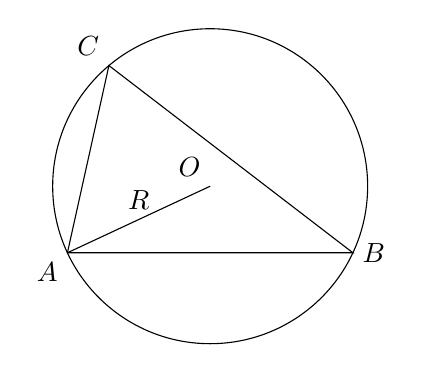
\begin{tikzpicture}
        \coordinate (O) at (0,0);
        \coordinate (B) at (-25:2cm);
        \coordinate (A) at (205:2cm);
        \coordinate (C) at (130:2cm);
        \coordinate (D) at (-90:2cm);
        
        \draw (O) circle (2cm);
        \draw (A) -- (B) -- (C) -- cycle;
        \node[right] at (B) {$B$};
        \node[below left] at (A) {$A$};
        \node[above left] at (C) {$C$};
        \node[above left] at (O) {$O$};
        \draw (A) -- node[above]{$R$} (O);
    \end{tikzpicture}
\end{center}
\subsection{Latihan Soal Teorema Garis Bagi}
\begin{enumerate}
    \item (OSK 2014) Diberikan segitiga $ABC$ dengan $AB = 360, BC = 240,$ dan $AC = 180$. Garis bagi dalam dan garis bagi luar dari $\angle CAB$ memotong $BC$ dan perpanjangan $BC$ berturut-turut di $P$ dan $Q$. Jari-jari lingkaran yang melalui titik-titik $A, P,$ dan $Q$ adalah \dots
\end{enumerate}
\subsection{Latihan Soal Teorema Garis Bagi}
\begin{enumerate}
    \item (OSK 2014) Diberikan segitiga $ABC$ dengan $AB = 360, BC = 240,$ dan $AC = 180$. Garis bagi dalam dan garis bagi luar dari $\angle CAB$ memotong $BC$ dan perpanjangan $BC$ berturut-turut di $P$ dan $Q$. Jari-jari lingkaran yang melalui titik-titik $A, P,$ dan $Q$ adalah \dots
    
    \item (OSK 2015) Pada segitiga $ABC$, garis tinggi $AD$, garis bagi $BE$ dan garis berat $CF$ berpotongan di satu titik. Jika panjang $AB = 4$ dan $BC = 5$, dan $CD = \frac{m^2}{n^2}$ dengan $m$ dan $n$ relatif prima, maka nilai dari $m - n$ adalah \ldots
\end{enumerate}
\subsection{Dalil Sinus dan Dalil Cosinus}
    Misalkan $ABC$ adalah suatu segitiga dengan $R$ adalah panjang jari-jari lingkaran luarnya.
\begin{center}
    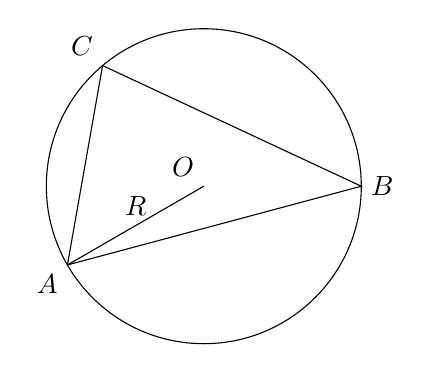
\begin{tikzpicture}
    \coordinate (O) at (0,0);
    \coordinate (B) at (0:2cm);
    \coordinate (A) at (210:2cm);
    \coordinate (C) at (130:2cm);
    
    \draw (O) circle (2cm);
    \draw (A) -- (B) -- (C) -- cycle;
    \node[right] at (B) {$B$};
    \node[below left] at (A) {$A$};
    \node[above left] at (C) {$C$};
    \node[above left] at (O) {$O$};
    \draw (A) -- node[above]{$R$} (O);
    \end{tikzpicture}
\end{center}
    \subsubsection{Dalil Sinus}
    $$\dfrac{BC}{\sin \angle A} = \dfrac{CA}{\sin \angle B}= \dfrac{AB}{\sin \angle C} = 2R$$
    
    \subsubsection{Dalil Cosinus}
    \begin{align*}
        AB^2 &= BC^2 + CA^2 - 2\cdot BC \cdot CA \cdot \cos \angle C\\
        BC^2 &= CA^2 + AB^2 - 2\cdot CA \cdot AB \cdot \cos \angle A\\
        CA^2 &= AB^2 + BC^2 - 2\cdot AB \cdot BC \cdot \cos \angle B
    \end{align*}
\subsection{Latihan Soal Dalil Sinus dan Cosinus}
\begin{enumerate}
    \item (OSK 2016) Pada segitiga $ABC$, titik $M$ terletak pada $BC$ sehingga $AB=7, AM=3, BM=5$, dan $MC=6$. Panjang $AC$ adalah \dots

    \item (OSK 2013) Misalkan $P$ adalah titik interior dalam daerah segitiga $ABC$ sehingga besar $\angle PAB = 10^\circ, \angle PBA = 20^\circ, \angle PCA = 30^\circ, \angle PAC=40^\circ$. Besar $\angle ABC = \dots$
    
    \item (Modifikasi OSK 2017) Pada sebuah lingkaran dengan pusat $O$, talibusur $AB$ berjarak 5 dari titik $O$ dan talibusur $AC$ berjarak $5\sqrt{2}$ dari titik $O$ dengan titik $A$ terletak di busur $BC$ yang lebih kecil ($A$ diantara $B$ dan $C$) Jika panjang jari-jari lingkaran 10, maka $BC^2=\dots$
\end{enumerate}
\subsection{Dalil Stewart}
    Pada segitiga $ABC$ dengan titik $D$ pada segmen $BC$, dimana $AB=c, BC=a, CA=b, AD=d, BD=m, CD=n$, maka berlaku
    $$BC \cdot AD^2 + BC \cdot BD \cdot CD = CA^2 \cdot BD + AB^2 \cdot CD$$
    atau $$ad^2+amn = b^2m+c^2n.$$

\subsection{Latihan Soal Dalil Stewart}
\begin{enumerate}
    \item (OSK 2016) Pada segitiga $ABC$, titik $M$ terletak pada $BC$ sehingga $AB=7, AM=3, BM=5$, dan $MC=6$. Panjang $AC$ adalah \dots
\end{enumerate}
\subsection{Latihan Soal Dalil Stewart}
\begin{enumerate}
    \item (OSK 2016) Pada segitiga $ABC$, titik $M$ terletak pada $BC$ sehingga $AB=7, AM=3, BM=5$, dan $MC=6$. Panjang $AC$ adalah \dots

    \item (HMMT 1999) Dalam segitiga $ABD$, $F$ berada pada segmen $AD$, $E$ berada pada sinar $BF$, $G$ berada pada segmen $BD$, dan $C$ adalah titik perpotongan dari $FG$ dan $ED$. Diketahui bahwa $AB = 15$, $BD = 18$, $AF = 15$, $DF = 12$, $BE = 24$, dan $CF = 17$. Temukan rasio $BG : FG$.
    % https://drive.google.com/drive/search?q=parent:0B-4OltLGFEDFeG92VENBbmdZODA%20type:pdf%20menelaus
\end{enumerate}
\subsection{Dalil Ceva}
Jika pada segitiga $ABC$, titik $D,E,F$ berturut-turut berada di segmen $BC$,$CA$,$AB$, maka 
$AD,BE,CF$ konkuren atau berpotongan di satu titik jika dan hanya jika $$\dfrac{AF}{FB} \cdot \dfrac{BD}{DC} \cdot \dfrac{CE}{EA} = 1.$$
\begin{center}
    \begin{tikzpicture}
    % titik-titik segitiga
    \coordinate[label=left:$A$]  (A) at (-1.5cm,-1.cm);
    \coordinate[label=right:$B$] (B) at (1.5cm,-1.0cm);
    \coordinate[label=above:$C$] (C) at (0.5cm,1.732cm);
    
    % pembuatan segitiga
    \draw (A) -- (B) -- (C) -- cycle;
    
    % titik-titik cevian
    \coordinate[label=below:$F$] (F) at ($(A)!0.7!(B)$);
    \coordinate[label=right:$D$] (D) at ($(B)!0.5!(C)$);
    \coordinate[label=left:$E$]  (E) at ($(C)!0.3!(A)$);
    
    % pembuatan cevian
    \draw (A) -- (D);
    \draw (B) -- (E);
    \draw (C) -- (F);
    \end{tikzpicture}
\end{center}
\subsection{Latihan Soal Dalil Ceva}
\begin{enumerate}
    \item (OSK 2015) Pada segitiga $ABC$, garis tinggi $AD$, garis bagi $BE$ dan garis berat $CF$ berpotongan di satu titik. Jika panjang $AB = 4$ dan $BC = 5$, dan $CD = \frac{m^2}{n^2}$ dengan $m$ dan $n$ relatif prima, maka nilai dari $m - n$ adalah \ldots
\end{enumerate}

\subsection{Dalil Menelaus}
Jika pada segitiga $ABC$, titik $P,Q,R$ berturut-turut berada pada garis (bisa di perpanjangan segmen) $BC$,$CA$, $AB$, maka $P,Q,R$ segaris jika dan hanya jika
$$\dfrac{AR}{RB} \cdot \dfrac{BP}{PC} \cdot \dfrac{CQ}{QA} = 1.$$
\begin{center}
    \begin{asy}
        unitsize(10);
        defaultpen(fontsize(8));
        pair P=(7,6), Q=(0,0), C=(10,0), A=(4,0), B=(6,8), R;
        draw((A)--(B)--(C)--cycle,blue+0.75);
        draw(P--R--Q--A);
        R=intersectionpoint(A--B,Q--P);
        dot(A^^B^^C^^P^^Q^^R);
        label("A",A,(0,-1));label("B",B,(1,0));label("C",C,(1,0));label("P",P,(1,1));label("Q",Q,(-1,0));label("R",R,(-1,1));
    \end{asy}
\end{center}
\subsection{Latihan Soal Dalil Menelaus}
\begin{enumerate}
    \item Dalam segitiga $ABD$, $F$ berada pada segmen $AD$, $E$ berada pada sinar $BF$, $G$ berada pada segmen $BD$, dan $C$ adalah titik perpotongan dari $FG$ dan $ED$. Diketahui bahwa $AB = 15$, $BD = 18$, $AF = 15$, $DF = 12$, $BE = 24$, dan $CF = 17$. Temukan rasio $BG : FG$.
    % https://drive.google.com/drive/search?q=parent:0B-4OltLGFEDFeG92VENBbmdZODA%20type:pdf%20menelaus

    \item (OSK 2022) Diberikan $ABC$ siku-siku sama kaki dengan $BC=AB$. Misalkan $L$ titik tengah $BC$ dan $P$ pada sisi $AC$ sehingga $BP \perp AL$. Jika $CP=30\sqrt{2}$, maka panjang $AB$ adalah \ldots

    \item Diberikan segitiga $ABC$ dengan panjang $BC = 36$. Misalkan $D$ adalah titik tengah $BC$ dan $E$ adalah titik tengah $AD$. Misalkan pula bahwa $F$ adalah perpotongan $BE$ dengan $AC$. Jika diketahui bahwa $AB$ menyinggung lingkaran luar segitiga $BFC$, hitunglah panjang $BF$.
\end{enumerate}
\subsection{Latihan Soal Dalil Menelaus}
\begin{enumerate}
    \item Dalam segitiga $ABD$, $F$ berada pada segmen $AD$, $E$ berada pada sinar $BF$, $G$ berada pada segmen $BD$, dan $C$ adalah titik perpotongan dari $FG$ dan $ED$. Diketahui bahwa $AB = 15$, $BD = 18$, $AF = 15$, $DF = 12$, $BE = 24$, dan $CF = 17$. Temukan rasio $BG : FG$.
    % https://drive.google.com/drive/search?q=parent:0B-4OltLGFEDFeG92VENBbmdZODA%20type:pdf%20menelaus

    \item (OSK 2022) Diberikan $ABC$ siku-siku sama kaki dengan $BC=AB$. Misalkan $L$ titik tengah $BC$ dan $P$ pada sisi $AC$ sehingga $BP \perp AL$. Jika $CP=30\sqrt{2}$, maka panjang $AB$ adalah \ldots

    \item Diberikan segitiga $ABC$ dengan panjang $BC = 36$. Misalkan $D$ adalah titik tengah $BC$ dan $E$ adalah titik tengah $AD$. Misalkan pula bahwa $F$ adalah perpotongan $BE$ dengan $AC$. Jika diketahui bahwa $AB$ menyinggung lingkaran luar segitiga $BFC$, hitunglah panjang $BF$.
\end{enumerate}
\subsection{Dalil Ptolemy}
    Diketahui sebuah segiempat siklis $ABCD$ maka berlaku
    $$AB \cdot CD + BC \cdot DA = AC \cdot BD.$$

\begin{center}
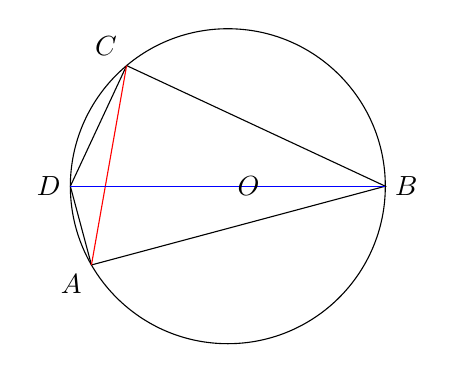
\begin{tikzpicture}
\coordinate (O) at (0,0);
\coordinate (B) at (0:2cm);
\coordinate (A) at (210:2cm);
\coordinate (D) at (180:2cm);
\coordinate (C) at (130:2cm);

\draw (O) circle (2cm);

\draw (A) -- (B) -- (C) -- (D) -- cycle;
\draw[red] (A) -- (C);
\draw[blue] (B) -- (D);

\node[right] at (B) {$B$};
\node[below left] at (A) {$A$};
\node[left] at (D) {$D$};
\node[above left] at (C) {$C$};
\node[right] at (O) {$O$};
\end{tikzpicture}
\end{center}

\subsection{Latihan Soal Dalil Ptolemy}
\begin{enumerate}
    \item Diberikan sebuah segiempat siklis $ABCD$ dengan $ABC$ adalah segitiga sama sisi. Jika $AD=2$ dan $CD=3$, panjang $BD=\dots$
\end{enumerate}
\subsection{Latihan Soal Dalil Ptolemy}
\begin{enumerate}
    \item Diberikan sebuah segiempat siklis $ABCD$ dengan $ABC$ adalah segitiga sama sisi. Jika $AD=2$ dan $CD=3$, panjang $BD=\dots$
\end{enumerate}

\section{Referensi}
    \begin{enumerate}
        \item Hermanto, Eddy. 2011. Diktat Pembinaan Olimpiade Matematika Dasar.
    \end{enumerate}



